\subsection{\texorpdfstring{以 \(\mu\) 为基的测度的特征刻画}{以 mu 为基的测度的特征刻画}}

定理 2（Lebesgue--Nikodym）. --- 设 \(\mu\) 和 \(\nu\) 是 T 上的两个正测度。下列性质等价：

\begin{enumerate}
\def\labelenumi{\arabic{enumi})}
\item
  \(\nu\) 是以 \(\mu\) 为基的测度。
\item
  每个局部 \(\mu\) -可忽略集都是局部 \(\nu\) -可忽略的。
\item
  每个 \(\mu\) -可忽略紧集都是 \(\nu\) -可忽略的。
\end{enumerate}

明显地，1) 蕴涵 2)（命题 3 的推论 1），且 2) 蕴涵 3)。我们将证明 3) 蕴涵 1)。首先注意，若条件 3) 满足，则每个普遍可测且局部 \(\mu\) -可忽略的集 A 都是局部 \(\nu\) -可忽略的；因为 \(\nu^{\bullet}(\mathrm{A}) = \sup \nu(\mathrm{K})\) ，其中 K 取遍含于 A 中的紧集所成之集（ \(\S 1\) , No.~3, 命题 10, a) 及 Ch. IV, \(\S 4\) , No.~6, 定理 4 的推论 2）。接下来，我们建立两个引理。

引理 2. --- 设 \(\alpha\) 是 T 上的一个有界正测度，\(\beta\) 是 T 上的一个实测度，满足 \(|\beta| \leqslant M\alpha\) ，其中 M 是一个正常数。则存在一个实函数 \(u\) ，它是 \(\alpha\) -可积的，使得 \(\beta = u \cdot \alpha\) 。

设 \(g\) 是空间 \(\mathcal{L}_{\mathbf{R}}^{2}(\mathrm{T},\alpha)\) 的一个元素；\(g\) 是 \(\beta\) -可测的，且 \(\int^{\bullet}|g|^2 d|\beta| \leqslant \mathrm{M}\int^{\bullet}|g|^2 d\alpha < +\infty\) 。因此函数 \(g\) 属于 \(\mathcal{L}^2 (\mathrm{T},|\beta|)\) ，而且也属于 \(\mathcal{L}^1 (\mathrm{T},|\beta|)\) ，因为 \(\beta\) 是有界的。由 Cauchy-Schwarz 不等式，

\[
| \beta (g) | ^ {2} \leqslant \left(\int | g | d | \beta |\right) ^ {2} \leqslant \left(\int d | \beta |\right) \left(\int | g | ^ {2} d | \beta |\right) \leqslant \mathrm{M} ^ {2} \alpha (1) \alpha (| g | ^ {2}).
\]

于是映射 \(g \mapsto \beta(g)\) 是 \(\mathcal{L}^2(\mathrm{T},\alpha)\) 上的一个连续线性形式。由于与 \(\mathcal{L}^2(\mathrm{T},\alpha)\) 相伴的 Hausdorff 空间是 Hilbert 空间，故存在（TVS, Ch. V, §1, No.~7, 定理 3）一个实函数 \(u \in \mathcal{L}^2(\mathrm{T},\alpha)\) （因而也属于 \(\mathcal{L}^1(\mathrm{T},\alpha)\) ），使得 \(\beta(g) = \alpha(ug)\) 对每个 \(g \in \mathcal{L}^2(\mathrm{T},\alpha)\) 都成立。把这个关系式应用于 \(g \in \mathcal{K}(\mathrm{T})\) ，即见 \(\beta = u\cdot \alpha\) 。

引理 3. --- 设正测度 \(\nu\) 使得每个 \(\mu\) -可忽略紧集都是 \(\nu\) -可忽略的。用 \(\mathfrak{K}\) 表示由具有下列性质的紧子集 \(K\) （\(T\) 中的）组成的集：

\begin{enumerate}
\def\labelenumi{(\arabic{enumi})}
\setcounter{enumi}{10}
\tightlist
\item
  存在一个常数 \(M \geqslant 0\) ，使得 \(\varphi_{K} \cdot \nu \leqslant M \varphi_{K} \cdot \mu\) 。此时集 K 在 T 中是 \(\mu\) -稠密的。
\end{enumerate}

若 K 满足 (11)，且 A 是含于 K 中的 Borel 集，则由命题 8 立即得出 \(\varphi_{\mathrm{A}} \cdot \nu \leqslant \mathrm{M}\varphi_{\mathrm{A}} \cdot \mu\) ；由此推出，K 与 \(K'\) （\(\mathfrak{K}\) 的两个元素）之并属于 \(\mathfrak{K}\) ，因为 \(\varphi_{\mathrm{K} \cup \mathrm{K}'} = \varphi_{\mathrm{K}} + \varphi_{\mathrm{A}}\) ，其中 \(\mathrm{A} = \mathrm{K}' \cap \mathbb{C}\mathrm{K}\) 。为建立引理，只须证明每个使 \(\mu(\mathrm{L}) > 0\) 的紧集 L 都包含一个紧集 \(\mathrm{K} \in \mathfrak{K}\) ，使得 \(\mu(\mathrm{K}) > 0\) （Ch. IV, §5, No.~8, 命题 12）。选取数 \(\mathrm{M} > \nu(\mathrm{L}) / \mu(\mathrm{L})\) ，并对有界正测度 \(\alpha = \varphi_{\mathrm{L}} \cdot (\nu + \mathrm{M}\mu)\) 与测度 \(\beta = \varphi_{\mathrm{L}} \cdot (\nu - \mathrm{M}\mu)\) 应用引理 1。如有必要，把函数 \(u\) （使 \(\beta = u \cdot \alpha\) 者）换成一个与它 \(\alpha\) -几乎处处相等的函数，就可以假设 \(u\) 是普遍可测的（§3, No.~4, 命题 7）且在 L 之外为零。由 \(t \in \mathrm{T}\) （使 \(u(t) < 0\) 者）组成的集 H 含于 L，它不可能是 \(\mu\) -可忽略的；因为否则它将是 \(\nu\) -可忽略的（由定理 2 证明开头的注记），从而是 \(\alpha\) -可忽略的，于是将有 \(\beta(\mathrm{L}) > 0\) ，这与 M 的选取相矛盾。设 K 是含于 H 中的一个紧集，使得 \(\mu(\mathrm{K}) > 0\) ；让我们证明 \(\mathrm{K} \in \mathfrak{K}\) ，这就将建立引理。由命题 8，

\[
\varphi_ {\mathrm{K}} \cdot (\nu - \mathrm{M} \mu) = \varphi_ {\mathrm{K}} \cdot \beta = \varphi_ {\mathrm{K}} \cdot (u \cdot \alpha) = (\varphi_ {\mathrm{K}} u) \cdot \alpha .
\]

函数 \(\varphi_{\mathbf{K}}u\) 是负的，因此确实有 \(\varphi_{\mathbf{K}}\cdot \nu \leqslant \mathrm{M}\varphi_{\mathbf{K}}\cdot \mu\) 。

现在来完成定理 2 的证明。假设条件 3) 成立，并按引理 3 那样定义 \(\mathfrak{K}\) 。设 \((\mathrm{K}_{\alpha})_{\alpha \in \mathbf{A}}\) 是 \(\mathfrak{K}\) 中两两不相交元素组成的一个局部可数族，使得集 \(\mathrm{N} = \mathrm{T} - \bigcup_{\alpha \in \mathbf{A}} \mathrm{K}_{\alpha}\) 是局部 \(\mu\) -可忽略的（Ch. IV, §5, No.~9, 命题 14）；由于族 \((\mathrm{K}_{\alpha})\) 是局部可数的，N 是普遍可测的，从而是局部 \(\nu\) -可忽略的。置 \(\mu_{\alpha} = \varphi_{\mathrm{K}_{\alpha}} \cdot \mu\) ，\(\nu_{\alpha} = \varphi_{\mathrm{K}_{\alpha}} \cdot \nu\) ；由于诸函数 \(\varphi_{\mathrm{K}_{\alpha}}\) 构成一个局部可数族，其和关于 \(\mu\) 与关于 \(\nu\) 都局部几乎处处等于 1 ，命题 6 蕴涵 \(\mu = \sum_{\alpha \in \mathbf{A}} \mu_{\alpha}\) ，\(\nu = \sum_{\alpha \in \mathbf{A}} \nu_{\alpha}\) 。另一方面，由 \(\mathfrak{K}\) 的定义，对每个 \(\alpha\) 存在常数 \(\mathrm{M}_{\alpha}\) ，使得 \(\nu_{\alpha} \leqslant \mathrm{M}_{\alpha} \mu_{\alpha}\) ；于是引理 2 蕴涵存在一个函数 \(g_{\alpha}\) （可以假设它在 \(\mathrm{K}_{\alpha}\) 之外为零且是正的）（命题 3 的推论 3），使得 \(\nu_{\alpha} = g_{\alpha} \cdot \mu_{\alpha}\) 。因此（No.~4, 命题 8）

\[
\nu_ {\alpha} = g _ {\alpha} \cdot \mu_ {\alpha} = g _ {\alpha} \cdot (\varphi_ {\mathrm{K} _ {\alpha}} \cdot \mu) = (g _ {\alpha} \varphi_ {\mathrm{K} _ {\alpha}}) \cdot \mu = g _ {\alpha} \cdot \mu .
\]

置 \(g = \sum_{\alpha \in A} g_{\alpha}\) ；由于族 \((g_{\alpha})\) 是局部可数的且族 \((\nu_{\alpha})\) 是可和的，命题 6 蕴涵 \(g\) 是局部 \(\mu\) -可积的，且 \(\nu = g \cdot \mu\) ，这就建立了定理。

推论 1. --- 设 N 是由以 \(\mu\) 为基的正测度组成的一个集，它有一个上确界 \(\nu\) （在 \(\mathcal{M}(\mathrm{T})\) 中）；则 \(\nu\) 是以 \(\mu\) 为基的测度。

命题 2 的推论允许化归到 N 是递增有向集的情形。于是，对每个局部 \(\mu\) -可忽略集 A ，依 §1, No.~4 的命题 11，有

\[
\nu^ {\bullet} (\mathrm{A}) = \sup _ {\lambda \in \mathcal {N}} \lambda^ {\bullet} (\mathrm{A}) = 0.
\]

因此定理 2 蕴涵 \(\nu\) 是以 \(\mu\) 为基的测度。

推论 2. --- 设 \(\nu\) 是 T 上的一个实测度。为使 \(\nu\) 属于由 \(\mu\) （在完全格序空间 \(\mathcal{M}(\mathrm{T})\) 中，Ch. II, §1, No.~5）生成的带，必须且只须 \(\nu\) 是以 \(\mu\) 为基的测度。

考虑 \(\nu^{+}\) 和 \(\nu^{-}\) ，立即化归到正测度 \(\nu\) 的情形（No.~2, 命题 2 的推论）。于是置 \(\nu_{n} = \inf(n\mu, \nu)\) ；\(\nu\) 属于由 \(\mu\) 生成的带当且仅当 \(\nu = \sup_{n} \nu_{n}\) （Ch. II, §1,

No.~5, 命题 6 的推论）。现在 \(\nu_{n}\) 被 \(n\mu\) 优超，故由定理 2 它是以 \(\mu\) 为基的测度；于是关系式 \(\nu = \sup_{n} \nu_{n}\) 蕴涵 \(\nu\) 是

以 \(\mu\) 为基的测度（推论 1）。反之，设 \(\nu\) 是以 \(\mu\) 为基的测度：\(\nu = g \cdot \mu\) ，其中 \(g\) 是局部 \(\mu\) -可积的正函数。此时 \(\nu_n = \inf(g, n) \cdot \mu\) （命题 2 的推论），且由 Lebesgue 定理（Ch. IV, §4, No.~3, 命题 4）立即得出 \(\nu = \sup_{n} \nu_n\) 。

推论 3. --- 设 \(\theta\) 是一个复测度；则存在一个普遍可测函数 \(v\) ，满足 \(|v| = 1\) ，使得 \(\theta = v \cdot |\theta|\) ，\(|\theta| = \overline{v} \cdot \theta\) 。

写 \(\theta = \theta_{1} - \theta_{2} + i(\theta_{3} - \theta_{4})\) ，其中 \(\theta_{1} = (\mathcal{R}\theta)^{+}\) ，\(\theta_{2} = (\mathcal{R}\theta)^{-}\) ，\(\theta_{3} = (\mathcal{I}\theta)^{+}\) ，\(\theta_{4} = (\mathcal{I}\theta)^{-}\) ；正测度 \(\theta_{i} (i = 1, 2, 3, 4)\) 被 \(|\theta|\) 优超（Ch. III, §1, No.~6, 公式 (17)），故由定理 2 都是以 \(|\theta|\) 为基的测度。由此推出，存在一个局部 \(|\theta|\) -可积函数 v ，使得 \(\theta = v \cdot |\theta|\) 。于是命题 2 给出关系 \(|\theta| = |v| \cdot |\theta|\) ，它蕴涵 \(|v| = 1\) 局部 \(|\theta|\) -几乎处处成立（命题 3 的推论 2）。最后，由命题 8，\(\overline{v} \cdot \theta = (v\overline{v}) \cdot |\theta| = |\theta|\) 。由于函数 v 只在一个局部 \(|\theta|\) -可忽略函数的范围内有定义，可以假设 v 是普遍可测的（§3, No.~4, 命题 7）且处处 \(|v| = 1\) 。

评注. --- 1) 设 \(\lambda\) 是一个正测度，\(v\) 是一个 \(\lambda\) -可测函数，满足 \(|v| = 1\) 局部 \(\lambda\) -几乎处处成立（这蕴涵 \(v\) 是局部 \(\lambda\) -可积的），并且 \(\theta = v \cdot \lambda\) 。命题 2 立即表明 \(\lambda = |\theta|\) ；换句话说，前一陈述的性质刻画了正测度 \(|\theta|\) 。

\begin{enumerate}
\def\labelenumi{\arabic{enumi})}
\setcounter{enumi}{1}
\tightlist
\item
  若 \(|\theta| \leqslant a\mu\) ，其中 \(\mu\) 是一个正测度且 \(a\) 是一个数 \(\geqslant 0\) ，则 \(\theta\) 是以 \(\mu\) 为基的测度。
\end{enumerate}

推论 4. --- 设 \(\rho\) 和 \(\theta\) 是两个复测度。为使存在一个局部 \(\theta\) -可积函数 \(u\) ，使得 \(\rho = u \cdot \theta\) ，必须且只须每个 \(\theta\) -可忽略紧集都是 \(\rho\) -可忽略的。

该条件显然是必要的。反之，设每个 \(\theta\) -可忽略紧集都是 \(\rho\) -可忽略的；定理 2 蕴涵存在一个局部 \(|\theta|\) -可积函数 g ，使得 \(|\rho| = g \cdot |\theta|\) 。另一方面，推论 3 蕴涵存在一个函数 \(v_{1}\) （相应地，\(v_{2}\) ），其绝对值为 1 且对测度 \(|\rho|\) （相应地，\(\theta\) ）可测，使得 \(\rho = v_{1} \cdot |\rho|\) （相应地，\(|\theta| = \overline{v}_{2} \cdot \theta\) ）。于是，由命题 8，\(\rho = u \cdot \theta\) ，其中 \(u = v_{1}g\overline{v}_{2}\) 。

推论 5. --- 设 \(\mu\) 和 \(\nu\) 是 T 上的两个正测度。定理 2 的条件 1)、2)、3) 也等价于下列条件：

\begin{enumerate}
\def\labelenumi{\arabic{enumi})}
\setcounter{enumi}{3}
\item
  对每个 \(\nu\) -可积数值函数 \(f \geqslant 0\) 及每个数 \(\varepsilon > 0\) ，存在一个 \(\delta > 0\) ，使得关系 \(0 \leqslant h \leqslant f\) 与 \(\int^{*} h d\mu \leqslant \delta\) 蕴涵 \(\int^{*} h d\nu < \varepsilon\) 。
\item
  对每个函数 \(g \in \mathcal{K}_{+}(\mathrm{T})\) 及每个数 \(\varepsilon > 0\) ，存在一个 \(\delta > 0\) ，使得对每个 \(h \in \mathcal{K}_{+}(\mathrm{T})\) （被 \(g\) 优超且满足 \(\int h d\mu \leqslant \delta\) 者），有 \(\int h d\nu \leqslant \varepsilon\) 。
\item
  对每个紧集 \(\mathbf{K} \subset \mathbf{T}\) 及每个数 \(\varepsilon > 0\) ，存在一个 \(\delta > 0\) ，使得关系 \(\mathbf{A} \subset \mathbf{K}\) 与 \(\mu^{*}(\mathbf{A}) \leqslant \delta\) 蕴涵 \(\nu^{*}(\mathbf{A}) \leqslant \varepsilon\) 。蕴涵关系 4) \(\Rightarrow 6) \Rightarrow 3)\) 是明显的。
\end{enumerate}

设存在一个有限函数 \(k \geqslant 0\) ，普遍可测且局部 \(\mu\) -可积，使得 \(\nu = k \cdot \mu\) ，让我们证明条件 4) 满足。设 f 是一个 \(\nu\) -可积函数 \(\geqslant 0\) ，并设 \(\varepsilon > 0\) 。对每个整数 \(n \geqslant 0\) ，设 \(A_{n}\) 是由 \(t \in T\) （使 \(k(t) \geqslant n\) 者）组成的集。诸函数 \(f\varphi_{A_{n}}\) 构成一个递减序列，被 f 优超且逐点趋于 0 ，因此存在一个 N ，使得 \(\int f\varphi_{A_{N}} d\nu \leqslant \varepsilon/2\) （Ch. IV, §4, No.~3, 命题 4）。若 h 是 T 上满足 \(0 \leqslant h \leqslant f\) 与 \(\int^{*} h d\mu \leqslant \varepsilon/2N\) 的函数，则

\[
\begin{array}{r l} & {\nu^ {*} (h) \leqslant \nu^ {*} (h \varphi_ {\mathrm {A_ {N}}}) + \nu^ {*} \big (h (1 - \varphi_ {\mathrm {A_ {N}}}) \big)} \\ & {\quad \leqslant \nu^ {*} (f \varphi_ {\mathrm {A_ {N}}}) + \mu^ {*} \big (h (1 - \varphi_ {\mathrm {A_ {N}}}) k \big)} \\ & {\quad \leqslant \frac {\varepsilon}{2} + \mathrm{N} \mu^ {*} (h) \leqslant \varepsilon .} \end{array}
\]

于是我们证明了条件 4) 与 6) 等价于定理 2 的诸条件。

明显地，4) 蕴涵 5)。最后，若条件 5) 满足，则 \(\nu\) 属于由 \(\mu\) 生成的带（Ch. II, §2, No.~2, 命题 5），从而以 \(\mu\) 为基（推论 2）。

概说. --- 对每个 \(\dot{f} \in \mathrm{L}_{\mathrm{loc}}^{1}(\mathrm{T}, \mu; \mathbf{R})\) ，置 \(\varphi(\dot{f}) = f \cdot \mu\) ，其中 \(f \in \dot{f}\) ；映射 \(\varphi\) 是线性的、递增的且单射的（命题 3 的推论 2），它在 \(\mathcal{M}(\mathrm{T})\) 中的像是由 \(\mu\) 生成的带 B（定理 2 的推论 2）。于是映射 \(\varphi\) 允许把 \(\mathrm{L}_{\mathrm{loc}}^{1}(\mathrm{T},\mu;\mathbf{R})\) 等同于 T 上的一个实测度空间；由于诸空间 \(\mathrm{L}_{\mathbf{R}}^{p}(\mathrm{T},\mu)\) 都是 \(\mathrm{L}_{\mathrm{loc}}^{1}(\mathrm{T},\mu;\mathbf{R})\) 的子空间，它们也可以等同于 \(\mathcal{M}(\mathrm{T})\) 的子空间。对复值函数与复测度有类似的考虑。注意，上面考虑的映射 \(\varphi\) 是 \(L_{loc}^{1}\) 与 B 的序向量空间结构之间的同构，但显然不是这些空间的拓扑向量空间结构之间的同构。

\pandocbounded{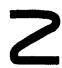
\includegraphics[keepaspectratio]{images/part002_ab1a0807.jpg}}

由于完全格序空间中的每个带本身都是完全格序空间（Ch. II, §1, No.~5），可见空间 \(L_{loc}^{1}\) 是完全格序的；但值得回忆的是，在 \(L_{loc}^{1}\) 中，一个由等价类组成的不可数族 \((\dot{f}_{\alpha})\) 的上确界不一定等同于诸函数 \(f_{\alpha}\) 的上包络的类。然而我们已看到，对于一个递增序列 \((f_{n})\) （由局部 \(\mu\) -可积函数组成），若其上包络 f 是局部 \(\mu\) -可积的，则 \(f \cdot \mu\) 是测度序列 \((f_{n} \cdot \mu)\) 在 \(\mathcal{M}(T)\) 中的上确界（命题 6 的推论）。

下面是定理 2 的推论 3 的一个有趣推论：

命题 9. --- 设 \(\theta\) 是一个有界复测度；为使 \(\theta\) 是正测度，必须且只须 \(\| \theta \| = \theta(1)\) 。

该条件显然是必要的。反之，设 \(\|\theta\|=\int d\theta\) ，并用 v 表示一个绝对值为 1 的 \(|\theta|\) -可测函数，使得 \(\theta=v\cdot|\theta|\) 。由于 \(\|\theta\|=\int d|\theta|\) （Ch. IV, §4, No.~7, 命题 12）且 \(\int d\theta=\int v\cdot d|\theta|\) （定理 1），假设蕴涵 \(\int(1-v)d|\theta|=0\) ，从而 \(\int\mathcal{R}(1-v)d|\theta|=0\) 。于是函数 \(\mathcal{R}(1-v)\) 是正的，故几乎处处为零，这蕴涵 v=1 几乎处处成立，证明完毕。

